%% LyX 2.0.4 created this file.  For more info, see http://www.lyx.org/.
%% Do not edit unless you really know what you are doing.
\documentclass[oneside,dutch]{amsart}
\usepackage[T1]{fontenc}
\usepackage[latin9]{inputenc}
\usepackage[a4paper]{geometry}
\geometry{verbose,tmargin=3cm,bmargin=3cm,lmargin=2cm,rmargin=2cm}
\setlength{\parskip}{\smallskipamount}
\setlength{\parindent}{0pt}
\usepackage{amsthm}
\usepackage{graphicx}
\graphicspath{{Figures/}}

\makeatletter

%%%%%%%%%%%%%%%%%%%%%%%%%%%%%% LyX specific LaTeX commands.
%% A simple dot to overcome graphicx limitations
\newcommand{\lyxdot}{.}


%%%%%%%%%%%%%%%%%%%%%%%%%%%%%% Textclass specific LaTeX commands.
\numberwithin{equation}{section}
\numberwithin{figure}{section}

\makeatother

\usepackage{babel}
\begin{document}

\title{Van der Waals en Wilson}


\author{N.G. Schultheiss}

\maketitle

\section{Inleiding}

Deze module bespreekt de werking van nevel- en bellenkamers. Dat zijn
detectoren waarmee kleine deeltjes, zoals stof of kosmische straling,
kunnen worden gedetecteerd. Beide detectoren gebruiken de overgang
van de vloeistof- naar de gasfase. Deze module wordt vervolgd met
de module ``Kosmische straling''.

Van der Waals deed onderzoek aan de overgang van de gas- en de vloeistoffase.
Wilson was als meteoroloog ge�nteresseerd in weer. Hij onderzocht
of hij wolken in een afgesloten kamer na kon maken. Tijdens dit onderzoek
ontdekte hij dat kosmische straling in deze ``Wilsonkamer'' gedetecteerd
werd.


\section{Van der Waals}

Van der Waals promoveerde op een proefschrift%
\footnote{Het gasmodel van Van der Waals beschrijft de overgang van de vloeibare-
naar de gasfase. De constanten geven de grootte-orde waarin dit gebeurt.
Ze zijn niet zo nauwkeurig bepaald als bijvoorbeeld de lichtsnelheid.
Verder is er nog veel onderzoek mogelijk op het gebied van de overgang
van vloeistof naar vaste stof.%
} genaamd: ``Over de continu�teit van den gas- en vloeistoftoestand''.
Dit proefschrift uit 1871 was in het Nederlands geschreven. In 1910
kreeg Van der Waals de Nobelprijs. In de tijd van Van der Waals was
men het er niet over eens dat stoffen uit atomen en moleculen waren
opgebouwd. De algemene gaswet $pV=nRT$ was wel bekend. Hierin geldt
$p$ is de druk van het gas in {[}$\frac{\mathrm{N}}{m^{2}}${]},
$V$ is het volume in {[}$\mathrm{m}^{3}${]}, $T$ is de temperatuur
in {[}K{]}, $n$ is de hoeveelheid gas in {[}mol{]} en $R$ is de
algemene gasconstante. 

Van der Waals breidde deze wet uit met twee idee�n: De deeltjes in
een gas namen een ruimte in en de deeltjes in een gas oefenen krachten
op elkaar uit. De algemene gaswet is nu te herschrijven als: 
\begin{equation}
\left(p+\frac{an^{2}}{V^{2}}\right)\left(V-nb\right)=nRT
\end{equation}


Dit is ook te schrijven als:

\begin{equation}
p=\frac{nRT}{V-nb}-\frac{an^{2}}{V^{2}}
\end{equation}


Zoals te zien is, gaat Van der Waals uit van het idee dat de ``plakkracht''
tussen de gasmoleculen een extra druk in het gas genereert. De druk
tussen de gasmoleculen wordt dus iets groter dan de druk $p$ die
wie van buiten op het gas meten. Deze ``plakkracht '' is overigens
de eigenlijke Van der Waals kracht. Later heeft deze term in de scheikunde
een bredere lading gekregen. Verder moet het volume van de gasmoleculen
van het samendrukbaar volume van het gas worden afgetrokken.

Experimenteel is voor water te bepalen dat $a=0.55[\frac{\mathrm{N}\mathrm{m}^{4}}{\mathrm{mo}\mathrm{l}^{2}}]$
en $b=30,4*10^{-6}[\frac{\mathrm{m}^{3}}{\mathrm{mol}}]$. 

\begin{figure}[h]
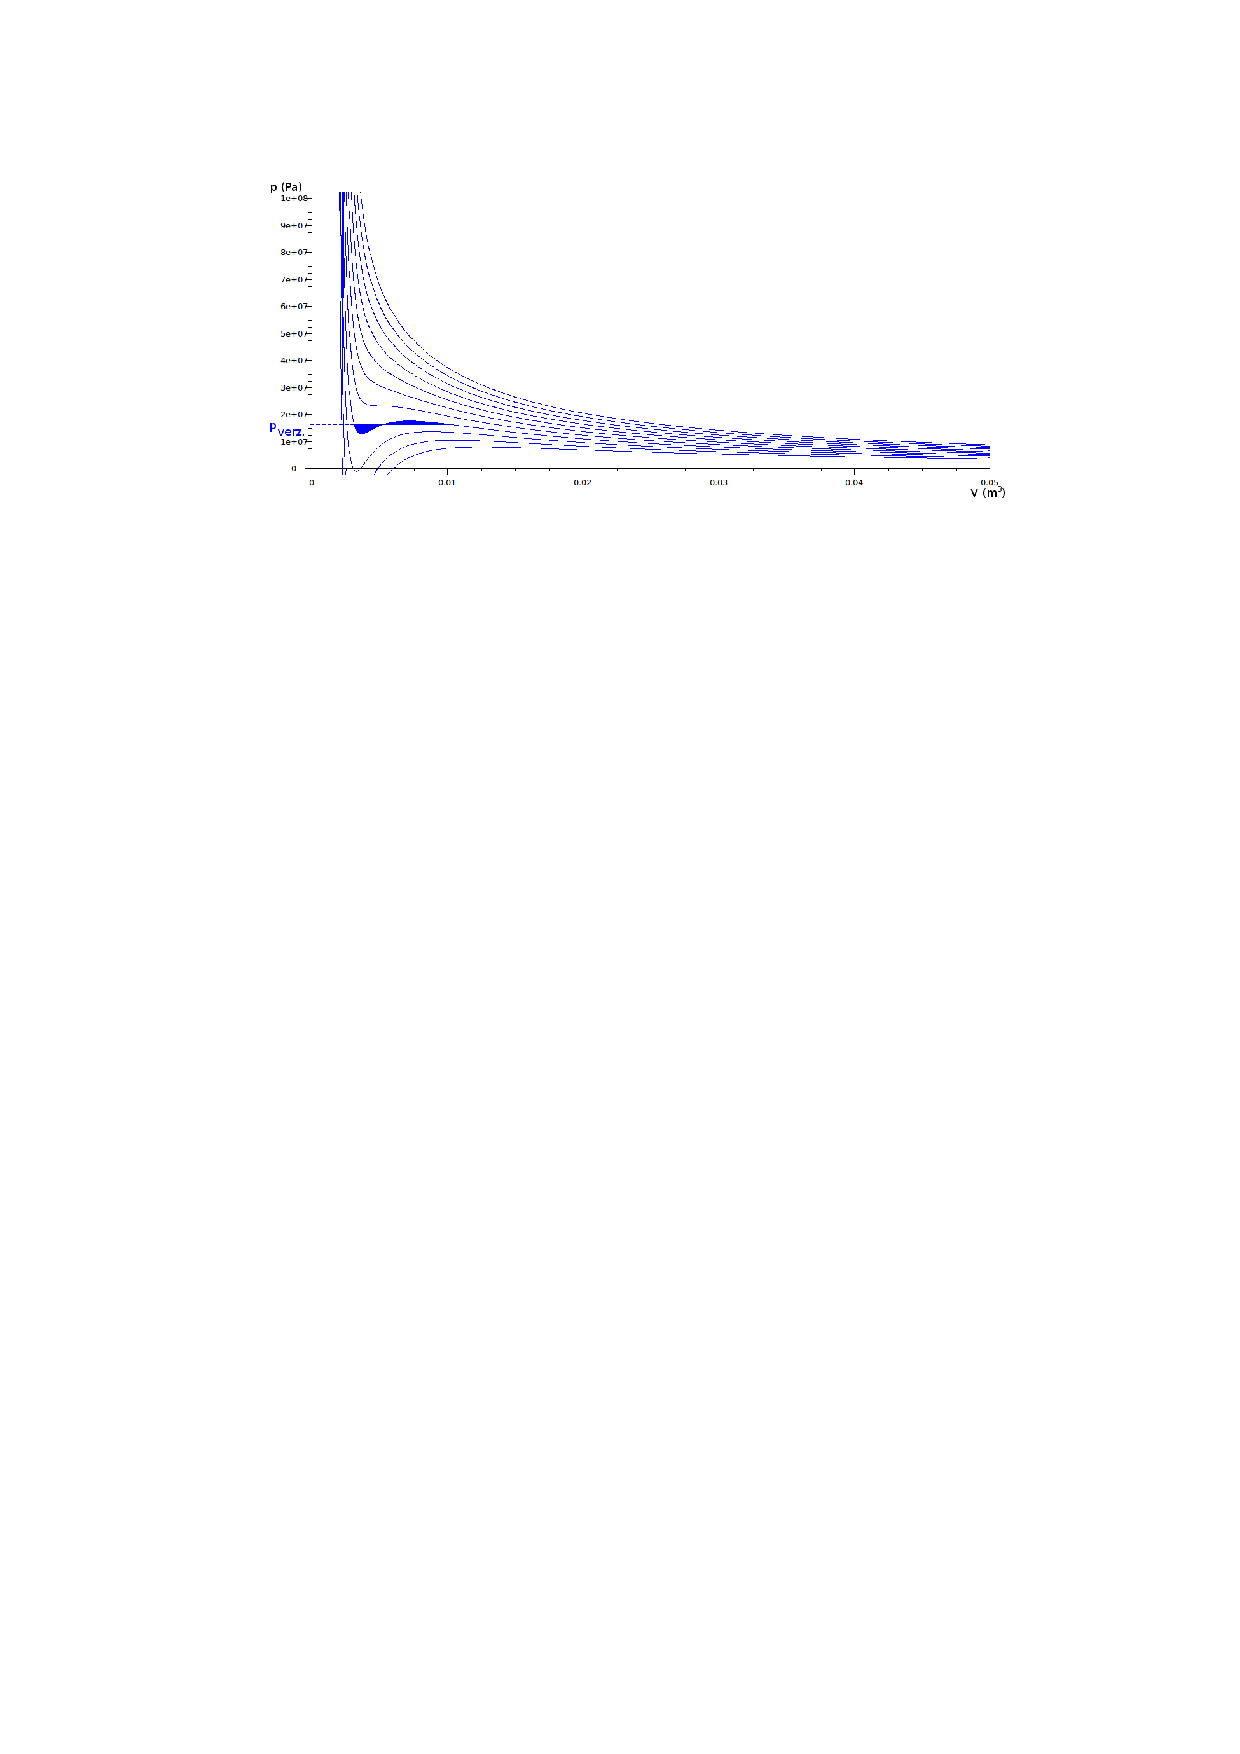
\includegraphics[scale=0.75]{vdwaals0}

\caption{De afhankelijkheid van druk en volume bij verschillende temperaturen}
\end{figure}


Zoals te zien is, wordt de functie voor een beperkte verzameling temperaturen
niet meer monotoon dalend. De slingering in de grafiek heeft te maken
met de faseverandering van vloeistof naar damp. 

Boven een bepaalde temperatuur wordt de functie wel monotoon dalend.
Hoe hoger de temperatuur boven de kritische temperatuur komt, hoe
meer het gas op een ideaal gas gaat lijken%
\footnote{Men spreekt van een ideaal gas als de toestanden te berekenen zijn
met de algemene gaswet.%
}. Boven deze kritische temperatuur vindt dan ook geen faseverandering
plaats. Over het algemeen spreekt men dan over een (niet ideaal) gas.
Bij temperaturen onder de kritische temperatuur vindt een faseovergang
plaats en spreekt men over een damp- of een vloeistoffase. 

Deze faseverandering onder de kritische temperatuur is te vinden met
de regel van Maxwell. Volgens deze regel is er een verzadigingsdruk.
Deze is te vinden door een lijn met de verzadigingsdruk te nemen zodat
het gesloten oppervlak boven de grafiek hetzelfde is als het gesloten
oppervlak onder de grafiek (donker aangegeven). In dit gebied komen
er dus naast elkaar een vloeistof- en een dampfase voor%
\footnote{Met de hefboomregel is de massa van de vloeistof te bepalen in de
evenwichtstoestand. De lijn tussen de vloeistoffase en de dampfase
scharniert als het ware om het punt (volume, verzadigingsdruk). De
massa van de vloeistof maal de arm naar de vloeistoffase is gelijk
aan de massa van de damp maal de arm naar de dampfase.%
}. 

Bij expansie van een vloeistof dalen we uit de vloeistoffase (links
in de grafiek) totdat de verzadigingsdruk is bereikt. Voor snelle
expansies in een zuivere vloeistof kan men onder de verzadigingsdruk
komen. We spreken dan van een oververhitte vloeistof. Als er dan een
deeltje door de vloeistof vliegt, zal dit deeltje een spoor dampbelletjes
maken. We hebben een bellenkamer. Is de vloeistof niet zuiver, dan
ontstaan er belletjes op de verontreining (stofjes)%
\footnote{Bij scheikunde voegt men daarom bij het verwarmen kooksteentjes (een
soort verontreiniging) aan een oplossing in een reageerbuis toe. Het
kookproces verloopt dan geleidelijker.%
}. 

Bij langzame compressie stijgt de druk tot de verzadigingsdruk. In
een zuivere stofvrije omgeving kunnen we boven de verzadigingsdruk
komen. We spreken van een onderkoelde damp. Als er in dit geval een
deeltje door de damp vliegt, zal dit deeltje een spoor druppeltjes
maken. We hebben een nevelkamer. In de praktijk werkt een nevelkamer
met een snelle expansie. Hierdoor daalt de temperatuur en komen we
ook in het gebied van de onderkoelde damp.

Een nevelkamer kan ook met diffusie werken, dan is er een continue
uitwisseling van de damp van een warmere naar een koudere omgeving.
De damp zal gaan condenseren als deze in een koudere omgeving komt.
Boven een nevellaag zijn spoortjes te zien. Hier vindt het condenseren
eerder plaats rond verstoringen zoals kosmische straling.


\section{Nevelkamers}

De nevelkamer volgens Wilson bestaat uit een messing cilinder met
een diameter van ongeveer 15cm. Hierin zit een zuiger ongeveer 3cm
onder een glazen deksel. In deze ruimte bevindt zich een verzadigde
damp. De zuiger kan plotseling naar beneden getrokken worden door
de ruimte onder de zuiger te verbinden met luchtledige bol met een
inhoud van ongeveer $2\mathrm{dm^{3}}$. 


\paragraph*{Opdracht 1:}

\emph{In Engeland worden andere eenheden gebruikt dan op het continent.
De Engelsen hebben ook eigen maten zoals , inch, foot, yard, mile,
gallon en pound. Ze zijn dan ook niet door Napoleon bezet geweest
en volgen ten dele het decimale stelsel. Er gaan bijvoorbeeld 12 inch
in 1 foot. Beredeneer welke afmeting Wilson waarschijnlijk gebruikt
heeft.}

Hij vond dat er geen nevel onstond als het volume minder dan 1,25
maal zo groot werd. Neemt het volume iets meer toe dan ontstaat er
een fijne neerslag. Boven een toename van 1,38 onstaat er een dichte
mist.

In 1912 ontdekte Wilson dat geladen deeltjes sporen in de mist vormden
bij een volumetoename met een factor 1,31.

Een verbeterde versie van de nevelkamer werd gemaakt door Takeo Shimizu%
\footnote{Shimizu is een veelvoorkomende Japanse naam en is toevallig te vertalen
als 'zuiver water'.%
} in 1921 op het Cavendish laboratorium. Shimizu bouwde een oscillerende
nevelkamer met een diameter van ongeveer 6cm. De zuiger wordt hier
mechanisch op en neer bewogen. Dit kan met frequenties in de buurt
van 3Hz. Bij iedere expansie (volumetoename) is er nevel te zien.
We kunnen met deze nevelkamer dus waarnemingen met een frequentie
van 3Hz doen%
\footnote{Het is wellicht mogelijk om een dergelijke nevelkamer uit aangepaste
bromfietsonderdelen en een electromotor samen te stellen. Het bouwen
van een dergelijke nevelkamer lijkt mij een goed onderwerp voor een
profielwerkstuk.%
}.


\paragraph*{Opdracht 2:}

\emph{Ontwerp een opstelling volgens het principe van Shimizu. We
gaan uit van een 4takt scootermotor met een inhoud van $50\mathrm{cm^{3}}$.
Hoe groot wordt het totale volume waarin we de nevel proberen te maken? }

http://jnm.snmjournals.org/cgi/content/full/44/8/1362


\section{Adiabatische expansie}

In het geval van een isotherm proces (de temperatuur is dan constant)
voldoen de toestanden van het gas aan $pV=constant$ of $pV=nRT$.
Ieder molecule krijgt nu een hoeveelheid energie die afhangt van $\frac{R}{N_{A}}=k$.
Deze nieuwe constante $k$ wordt de Boltzmann-constante genoemd, $N_{A}$
is het getal van Avogadro en geeft het aantal moleculen in een mol.

Een adiabatisch proces is een proces waarbij geen warmte wordt af-
of toegevoerd. Voor tweeatomige moleculen zoals lucht geldt dat $p^{2}=cT^{7}$.
Hierna wordt dit voor de volledigheid afgeleid. 

Een warmtestroom is te beschouwen als een overdracht van energie van
het ene naar het andere systeem. Als een gas door middel van een zuiger
wordt ge�xpandeerd, verricht de kracht van het gas arbeid op de zuiger.
Omdat arbeid ook een verandering van energie is, neemt de inwendige
energie en daarmee de temperatuur van het gas af. 

De inwendige energie van een ideaal gas wordt gevormd door het verplaatsen,
draaien en eventueel het trillen van de gasmoleculen.

Een ��natomig gasmolecuul kan vrij bewegen en heeft daarmee drie vrijheidsgraden.
\begin{itemize}
\item De plaats: x, y en z. 
\end{itemize}
Lucht bestaat hoofdzakelijk uit tweeatomige gasmoleculen. Dergelijke
moleculen hebben ook een richting, dit geeft twee nieuwe vrijheidsgraden.
\begin{itemize}
\item De hoek, deze geeft een hoek in het (x,y)-vlak en een hoek ten opzicht
van de z-as.
\end{itemize}
Er zijn voor een tweeatomig gas dus een aantal mogelijke energi�n:
\begin{itemize}
\item Drie vrijheidsgraden voor de plaats, ieder met hun eigen bewegingsenergie.
\item Twee vrijheidsgraden voor de hoek, ook met hun eigen bewegingsenergie.
\end{itemize}
Een tweeatomig gasmolecuul heeft dus 5 vrijheidsgraden. Iedere vrijheidsgraad
krijgt een energie van $\frac{1}{2}kT$. Als er geen arbeid wordt
verricht, moeten we $\frac{5}{2}k\triangle T$ aan het gas aan het
gas toevoeren om het te verwarmen. Bij een constante druk wordt dit
door de verrichte arbeid $\frac{7}{2}k\triangle T$. 

Bij een adiabatisch proces wordt er geen warmte toegevoerd, de inwendige
energie af neemt als er arbeid wordt verricht. We krijgen nu:

\begin{equation}
pV^{\frac{7}{5}}=c_{1}
\end{equation}


Voor iedere toestand geldt $\frac{pV}{T}=constant$. Dit is ook te
schrijven als:

\begin{equation}
V=\frac{c_{2}T}{p}
\end{equation}


Substitutie geeft:

\begin{equation}
p\left(\frac{c_{2}T}{p}\right)^{\frac{7}{5}}=c_{1}\Rightarrow\frac{T^{\frac{7}{5}}}{p^{\frac{2}{5}}}=\frac{c_{1}}{c_{2}}=\frac{1}{c}\Rightarrow p^{2}=cT^{7}
\end{equation}



\section{Nevelvorming}

Een van der Waals gas heeft een fase verandering als we onder de kritische
tempera\-tuur blijven. De tempera\-tuur waarbij deze faseverandering
optreedt, wordt het dauwpunt genoemd. De druk waarbij deze faseverandering
optreedt wordt de verzadigingsdruk genoemd. De verzadigingsdruk boven
water is te benaderen met%
\footnote{http://home.kpn.nl/vanadovv/Meteo.html%
}:

\begin{equation}
p_{verz.}=610.78e^{\frac{17,26t}{t+237,3}}
\end{equation}


Boven ijs is dit:

\begin{equation}
p_{verz.}=610,78e^{\frac{21,87t}{t+265.5}}
\end{equation}


Hierin wordt $t$ in $\mathrm{^{o}C}$ gegeven en $p_{verz.}$ in
Pa of $\frac{\mathrm{N}}{\mathrm{m}^{2}}$.

\begin{figure}[h]
\noindent \begin{centering}
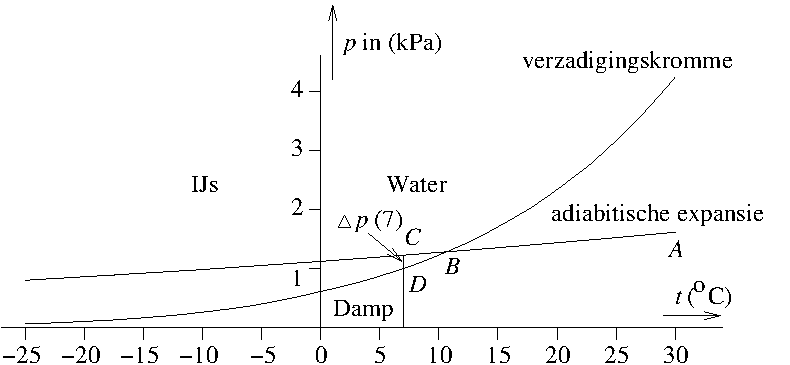
\includegraphics[scale=0.75]{dampkromme}
\par\end{centering}

\caption{Dampdruk / temperatuur}
\end{figure}


In figuur 5.1 is de dampdruk van water tegen de temperatuur te zien.
Daarnaast is een adiabatisch expansie-proces van punt $A$ via $B$
naar $C$ te zien. De relatieve luchtvochtigheid is voor iedere toestand
van dit proces te vinden door de druk van de adiabatische expansie
te delen door de verzadigingsdruk. In punt $B$ is de damp verzadigd.
De relatieve vochtigheid is dan 100\%. Onder deze temperatuur zal
het gas in eerste instantie langs de lijn van de adiabatische expansie
afkoelen. Helaas is de relatieve luchtvochtigheid dan meer dan 100\%
en is de damp oververzadigd. Op onregelmatigheden in de damp zal nu
condensatie optreden. Met wat geluk zijn er sporen van ge�oniseerde
lucht te zien. De gecondenseerde massa gedeeld door de massa bij $\mathrm{7^{o}C}$
is te vinden door $\triangle p(7)$ (tussen $C$ en $D$) te delen
door $p(7)$ (de hoogte tot $C$). 


\paragraph*{Opdracht :}

\emph{Met formule 4.1 is nu te onderzoeken hoeveel een gas, dat voornamelijk
uit tweeatomige moleculen bestaat, moet expanderen. Volgens Wilson
is de expansiefactor 1,31 om deeltjes waar te nemen. Welk drukverschil
onstaat er dan?}
\end{document}
